% ================================ L'IMPLEMENTAZIONE ====================================

\chapter{L'implementazione}

%TODO: Implementazione in C++
%TODO: Con gui e command line o solo gui.

%TODO: Volendo anche Java?

%TODO: Presenterò/Mostrerò due implementazioni una fatta specificamente per questo progetto in C++ e un'altra in Java che avevo fatto per altri progetti.
%TODO: Quella in C++ sarà più completa rispetto di quella in Java.

% =======================================================================================

% ---------------------------- SECTION: INTRODUZIONE ------------------------------------

\section{Introduzione}

\textsf{\small } %TODO: In questo capitolo, presenterò due implementazioni, una elaborata esclusivamente per questo progetto in C++ e un'altra in Java che avevo creato per altri progetti universitari. Quella in C++ risulterà più completa rispetto a quella in Java.

% ---------------------------- SECTION: IMPLEMENTAZIONE IN C++ --------------------------

\section{Implementazione in C++}

\textsf{\small } %TODO: Ho adottato C++23 per questo progetto. In esso sono presenti una interfaccia grafica e una applicazione da linea di comando, entrambe hanno le stesse operazioni.

%TODO: Inanzittutto, esibirò, le funzioni riguardanti la matematica di Galois di cui mi sono avvalso.

\subsection{Matematica di Galois}

\textsf{\small } %TODO: 

\begin{figure}[H]
	\centering
	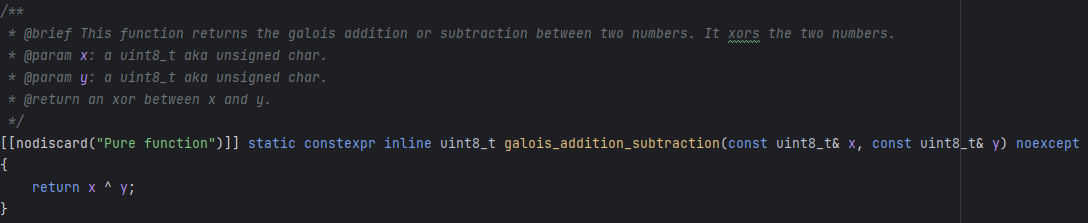
\includegraphics[width=1\textwidth, height=1\textheight, keepaspectratio]{./images/code/cpp/galois_math/galois_addition_subtraction.PNG}
	\caption{Addizione e sottrazione nel campo di Galois}
	\label{fig:galois_addition_subtraction}
\end{figure}

\textsf{\small } %TODO: 

\begin{figure}[H]
	\centering
	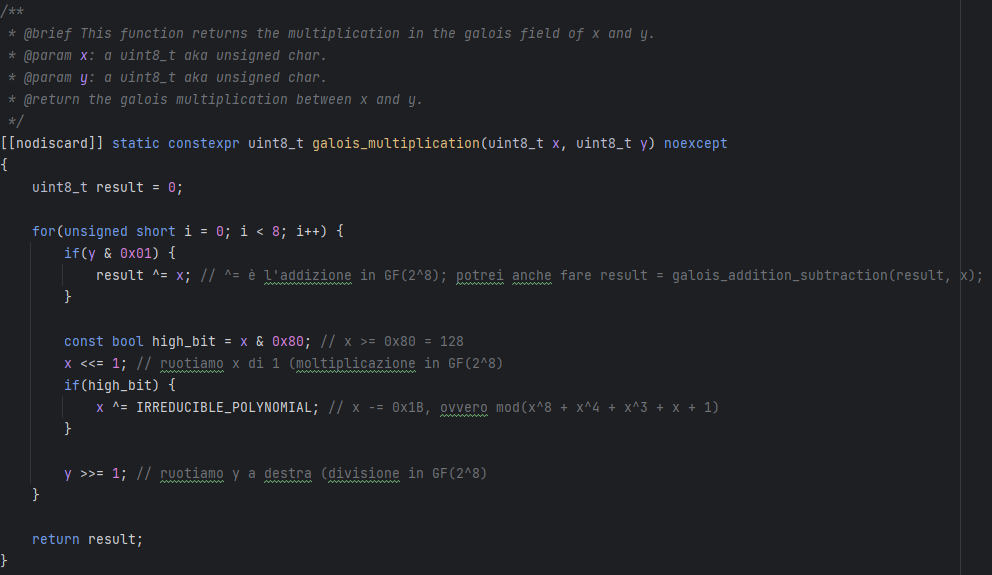
\includegraphics[width=1\textwidth, height=1\textheight, keepaspectratio]{./images/code/cpp/galois_math/galois_multiplication.PNG}
	\caption{Moltiplicazione nel campo di Galois}
	\label{fig:galois_multiplication}
\end{figure}

\textsf{\small } %TODO: 

\begin{figure}[H]
	\centering
	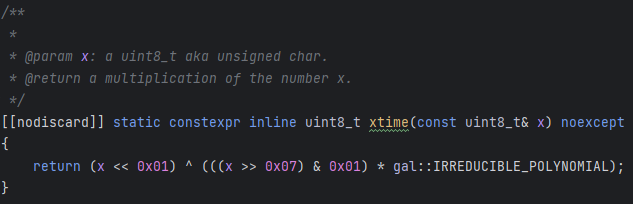
\includegraphics[width=1\textwidth, height=1\textheight, keepaspectratio]{./images/code/cpp/galois_math/xtime.PNG}
	\caption{Moltiplicazione nel campo di Galois 2}
	\label{fig:xtime}
\end{figure}

%TODO: Come prima cosa mostrerò l'implementazione dell'algoritmo di AES con tutte le varie operazioni all'interno di ogni round di AES, ovvero: add round key, sub bytes, shift rows e mix columns. Dopodiché presenterò la parte di Key Expansion, ovvero come vengono ottenute le chiavi per ogni round, anch'esso composto da queste fasi: rot word, sub word, rcon.

%\subsection{Cifratura} %TODO: uncomment?

\subsection{Add Round Key}

%TODO: immagine del codice.

\begin{figure}[H]
	\centering
	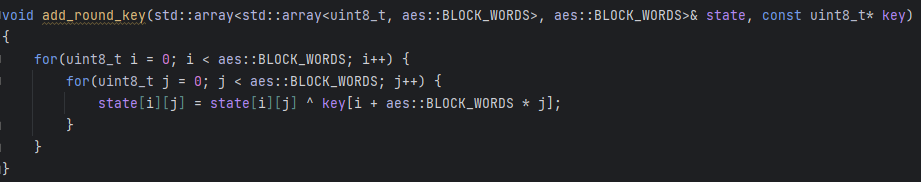
\includegraphics[width=1\textwidth, height=1\textheight, keepaspectratio]{./images/code/cpp/encryption/add_round_key.PNG}
	\caption{Add Round Key}
	\label{fig:add_round_key}
\end{figure}

\textsf{\small } %TODO:

\subsection{Sub Bytes}

\begin{figure}[H]
	\centering
	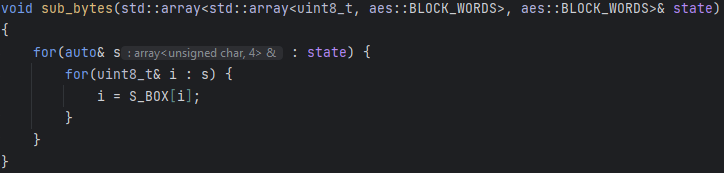
\includegraphics[width=1\textwidth, height=1\textheight, keepaspectratio]{./images/code/cpp/encryption/sub_bytes.PNG}
	\caption{Sub Bytes}
	\label{fig:sub_bytes}
\end{figure}

\textsf{\small } %TODO:

\subsection{Shift Rows}

\begin{figure}[H]
	\centering
	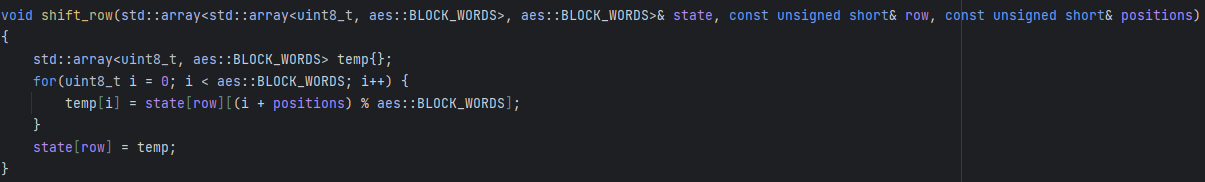
\includegraphics[width=1\textwidth, height=1\textheight, keepaspectratio]{./images/code/cpp/encryption/shift_row.PNG}
	\caption{Shift Row}
	\label{fig:shift_row}
\end{figure}

\textsf{\small } %TODO:

\begin{figure}[H]
	\centering
	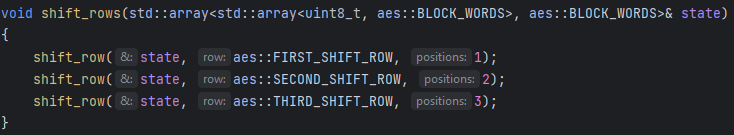
\includegraphics[width=1\textwidth, height=1\textheight, keepaspectratio]{./images/code/cpp/encryption/shift_rows.PNG}
	\caption{Shift Rows}
	\label{fig:shift_rows}
\end{figure}

\subsection{Mix Columns}

\textsf{\small } %TODO:

\begin{figure}[H]
	\centering
	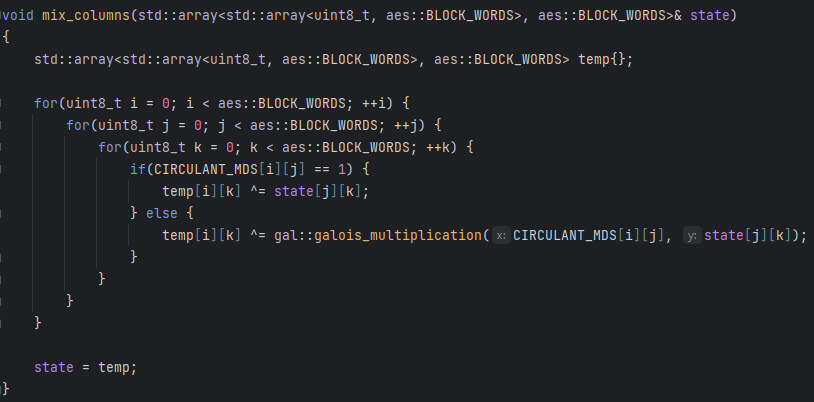
\includegraphics[width=1\textwidth, height=1\textheight, keepaspectratio]{./images/code/cpp/encryption/mix_columns.PNG}
	\caption{Mix Columns}
	\label{fig:mix_columns}
\end{figure}

%\subsection{Decifratura} %TODO: uncomment?

\subsection{Key Expansion}

\begin{figure}[H]
	\centering
	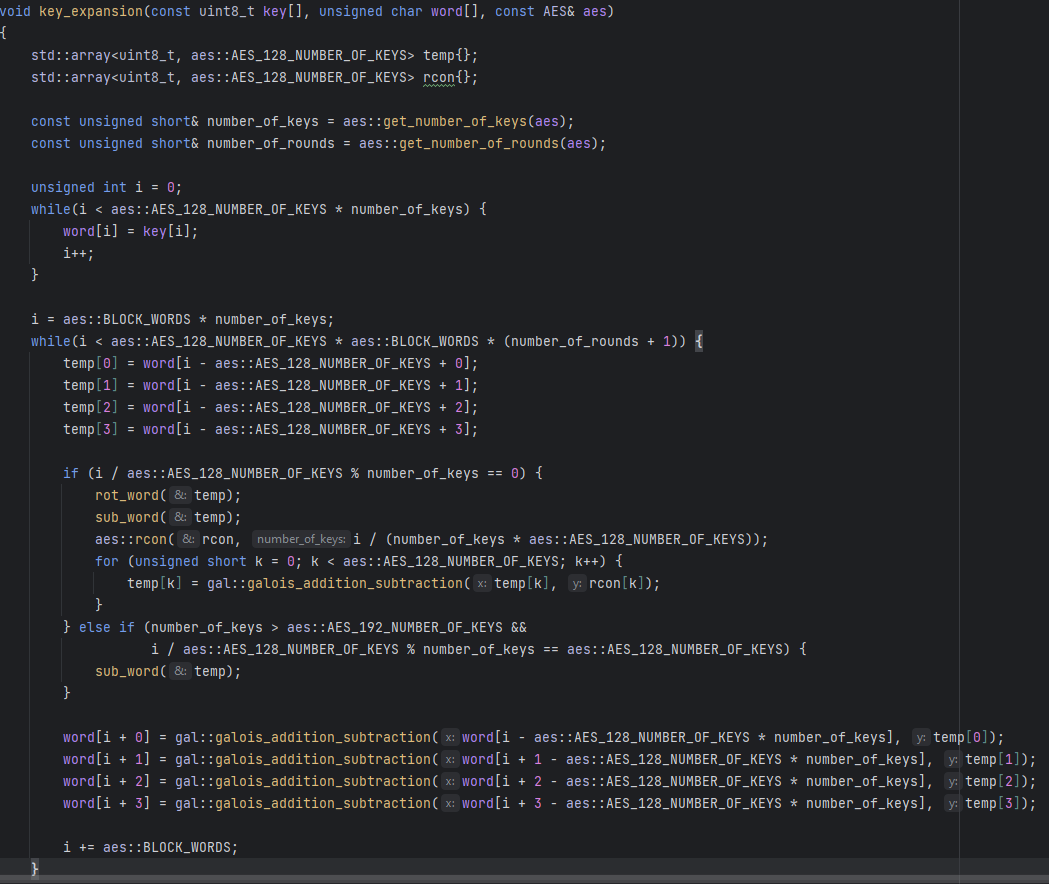
\includegraphics[width=1\textwidth, height=1\textheight, keepaspectratio]{./images/code/cpp/key_expansion/key_expansion.PNG}
	\caption{Key Expansion}
	\label{fig:key_expansion_code}
\end{figure}

\textsf{\small } %TODO:

\subsubsection{Rot Word}

\begin{figure}[H]
	\centering
	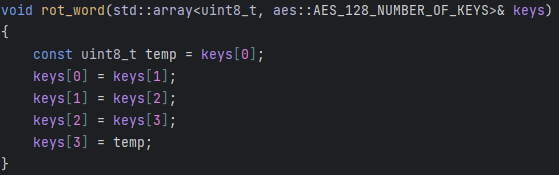
\includegraphics[width=1\textwidth, height=1\textheight, keepaspectratio]{./images/code/cpp/key_expansion/rot_word.PNG}
	\caption{Rot Word}
	\label{fig:rot_word}
\end{figure}

\textsf{\small } %TODO:

\subsubsection{Sub Word}

\begin{figure}[H]
	\centering
	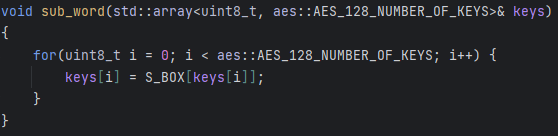
\includegraphics[width=1\textwidth, height=1\textheight, keepaspectratio]{./images/code/cpp/key_expansion/sub_word.PNG}
	\caption{Sub Word}
	\label{fig:sub_word}
\end{figure}

\textsf{\small } %TODO:

\subsubsection{Rcon}

\begin{figure}[H]
	\centering
	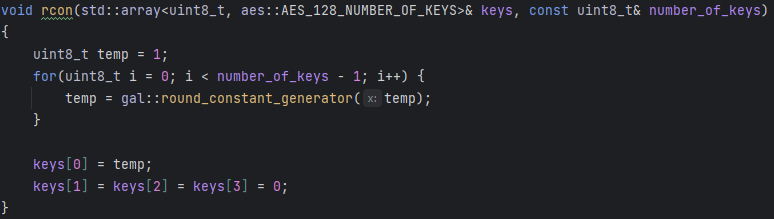
\includegraphics[width=1\textwidth, height=1\textheight, keepaspectratio]{./images/code/cpp/key_expansion/rcon.PNG}
	\caption{Rcon}
	\label{fig:rcon}
\end{figure}

\textsf{\small } %TODO:

\subsubsection{Xor Blocks} %TODO: uncomment?

%\textsf{\small } %TODO:

\subsection{Modes}

\textsf{\small } %TODO:

%TODO: subsection: Modes con codice? Questo si potrebbe fare.

\subsubsection{ECB}

\begin{figure}[H]
	\centering
	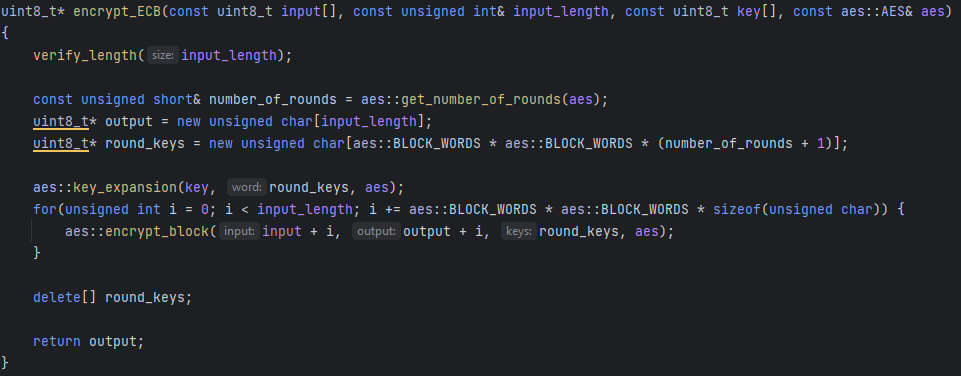
\includegraphics[width=1\textwidth, height=1\textheight, keepaspectratio]{./images/code/cpp/modes/encrypt_ECB.PNG}
	\caption{Cifratura ECB}
	\label{fig:encrypt_ECB}
\end{figure}

\textsf{\small } %TODO:

\begin{figure}[H]
	\centering
	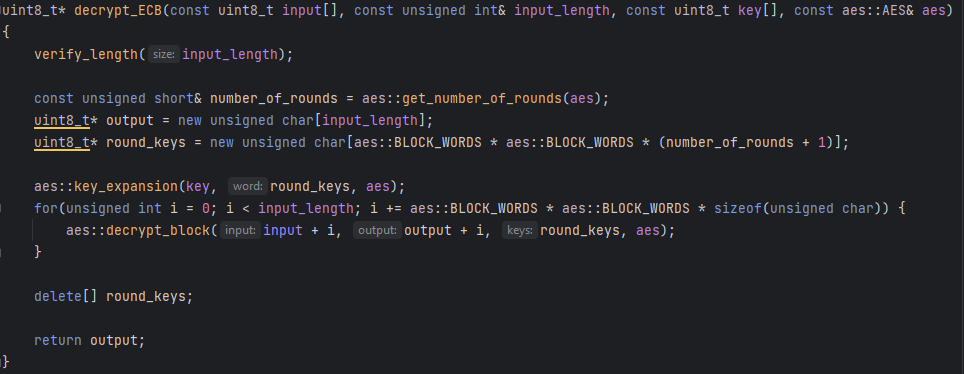
\includegraphics[width=1\textwidth, height=1\textheight, keepaspectratio]{./images/code/cpp/modes/decrypt_ECB.PNG}
	\caption{Decifrazione ECB}
	\label{fig:decrypt_ECB}
\end{figure}

\subsubsection{CBC}

\begin{figure}[H]
	\centering
	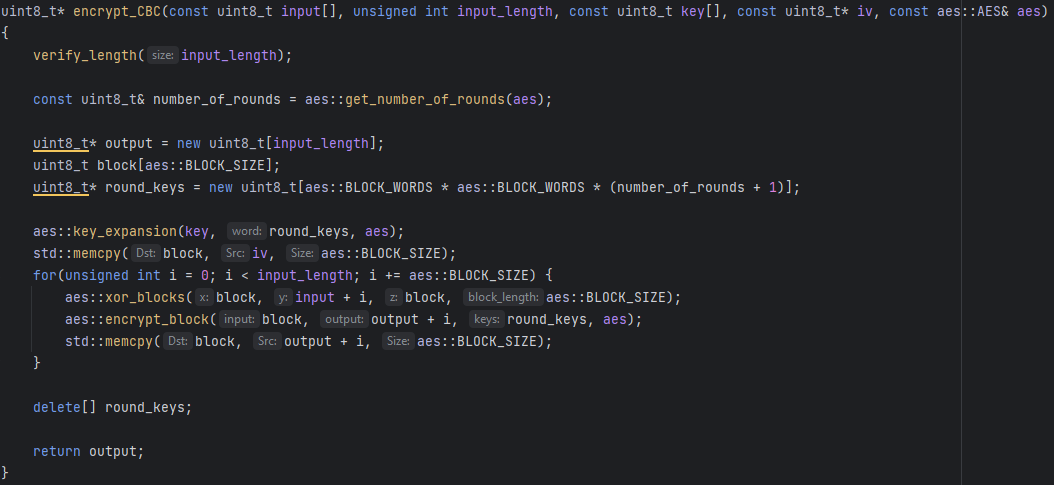
\includegraphics[width=1\textwidth, height=1\textheight, keepaspectratio]{./images/code/cpp/modes/encrypt_CBC.PNG}
	\caption{Cifratura CBC}
	\label{fig:encrypt_CBC}
\end{figure}

\textsf{\small } %TODO:

\begin{figure}[H]
	\centering
	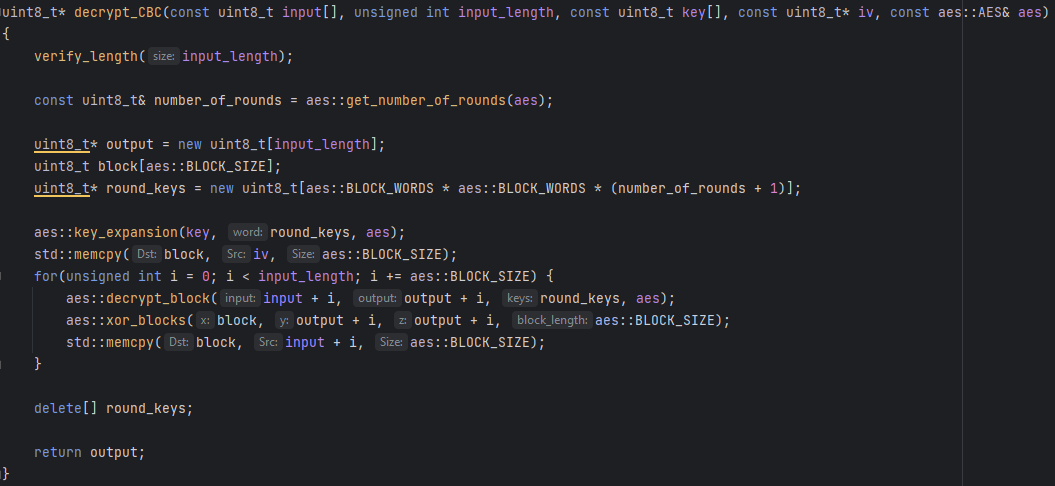
\includegraphics[width=1\textwidth, height=1\textheight, keepaspectratio]{./images/code/cpp/modes/decrypt_CBC.PNG}
	\caption{Decifrazione CBC}
	\label{fig:decrypt_CBC}
\end{figure}

\subsubsection{CFB}

\textsf{\small } %TODO:

\begin{figure}[H]
	\centering
	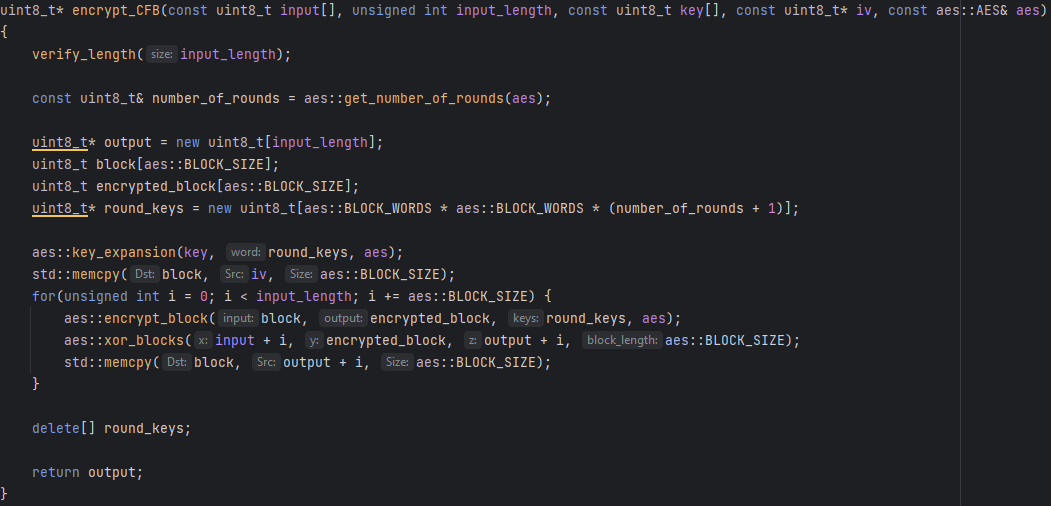
\includegraphics[width=1\textwidth, height=1\textheight, keepaspectratio]{./images/code/cpp/modes/encrypt_CFB.PNG}
	\caption{Cifratura CFB}
	\label{fig:encrypt_CFB}
\end{figure}

\textsf{\small }

\begin{figure}[H]
	\centering
	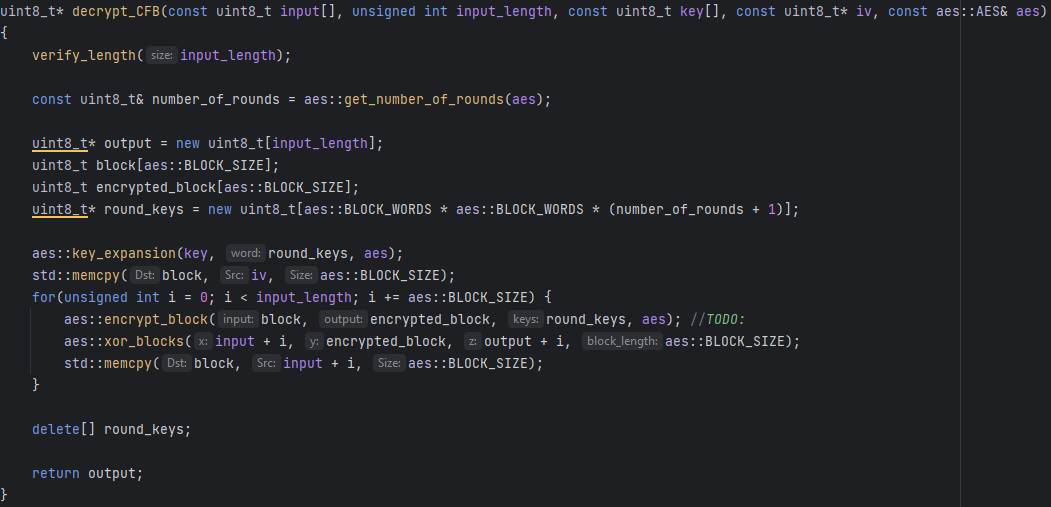
\includegraphics[width=1\textwidth, height=1\textheight, keepaspectratio]{./images/code/cpp/modes/decrypt_CFB.PNG}
	\caption{Decifrazione CFB}
	\label{fig:decrypt_CFB}
\end{figure}

\subsection{Paddings}

\textsf{\small } %TODO:

\begin{figure}[H]
	\centering
	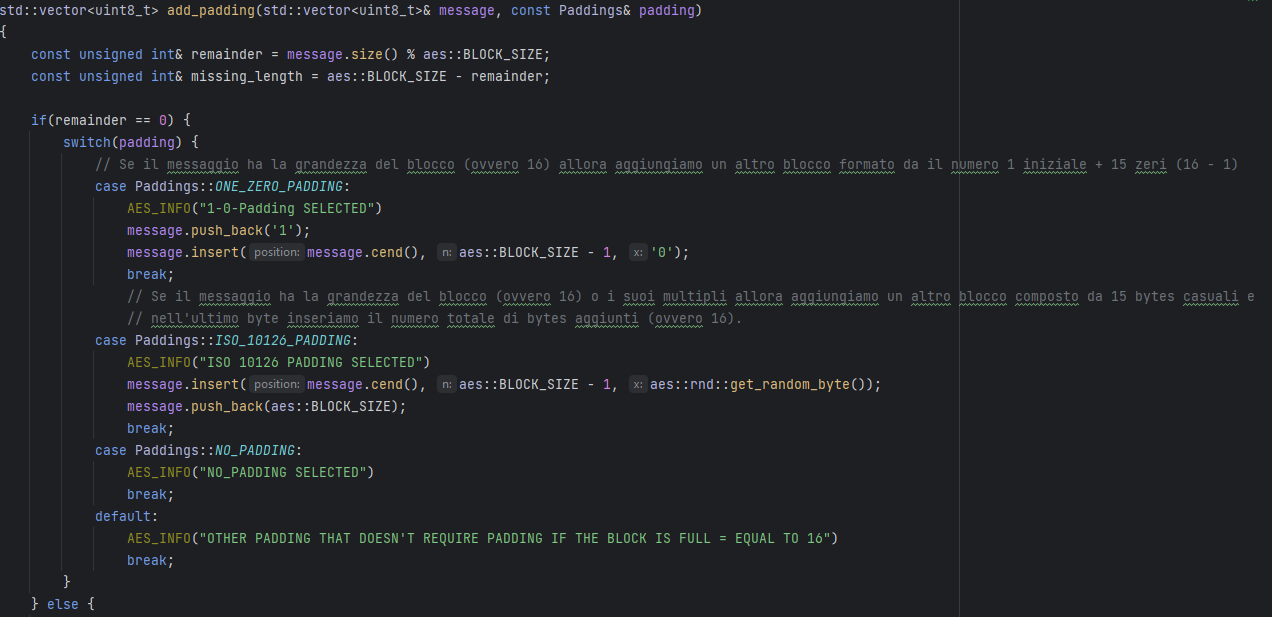
\includegraphics[width=1\textwidth, height=1\textheight, keepaspectratio]{./images/code/cpp/padding/add_padding0.PNG}
	\caption{Aggiunta del padding (1/2)}
	\label{fig:add_padding0}
\end{figure}

\begin{figure}[H]
	\centering
	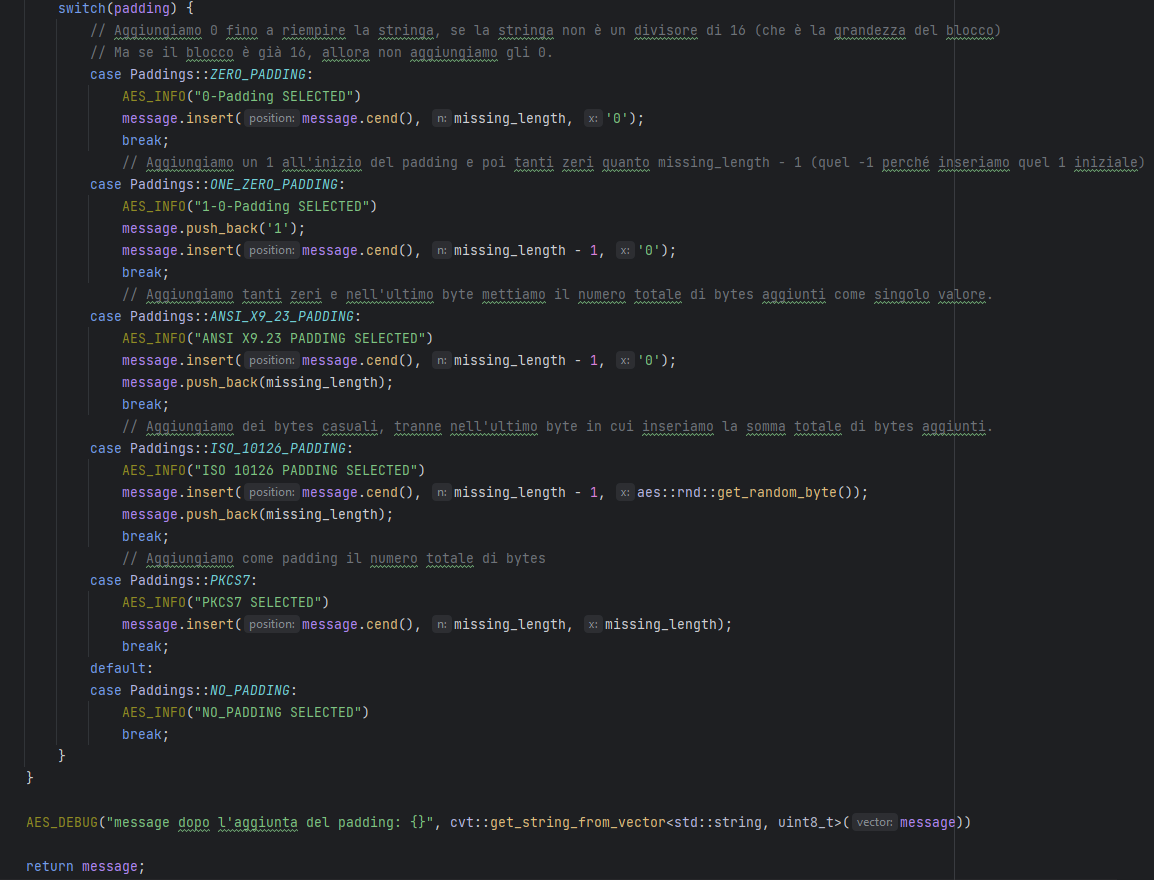
\includegraphics[width=1\textwidth, height=1\textheight, keepaspectratio]{./images/code/cpp/padding/add_padding1.PNG}
	\caption{Aggiunta del padding (2/2)}
	\label{fig:add_padding1}
\end{figure}

\textsf{\small }

\begin{figure}[H]
	\centering
	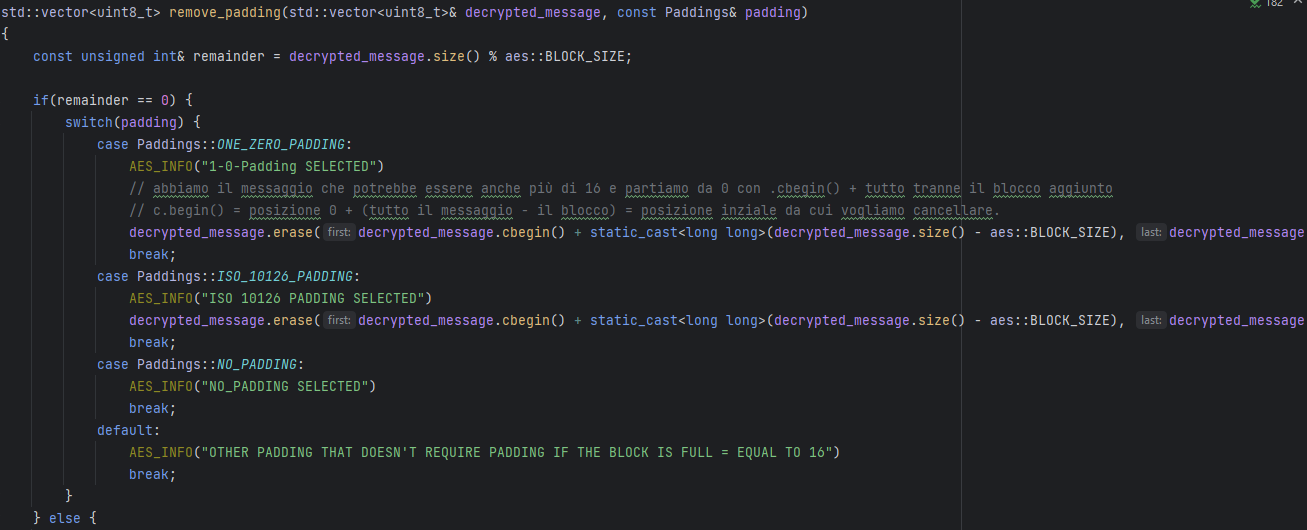
\includegraphics[width=1\textwidth, height=1\textheight, keepaspectratio]{./images/code/cpp/padding/remove_padding0.PNG}
	\caption{Rimozione del padding (1/2)}
	\label{fig:remove_padding0}
\end{figure}

\begin{figure}[H]
	\centering
	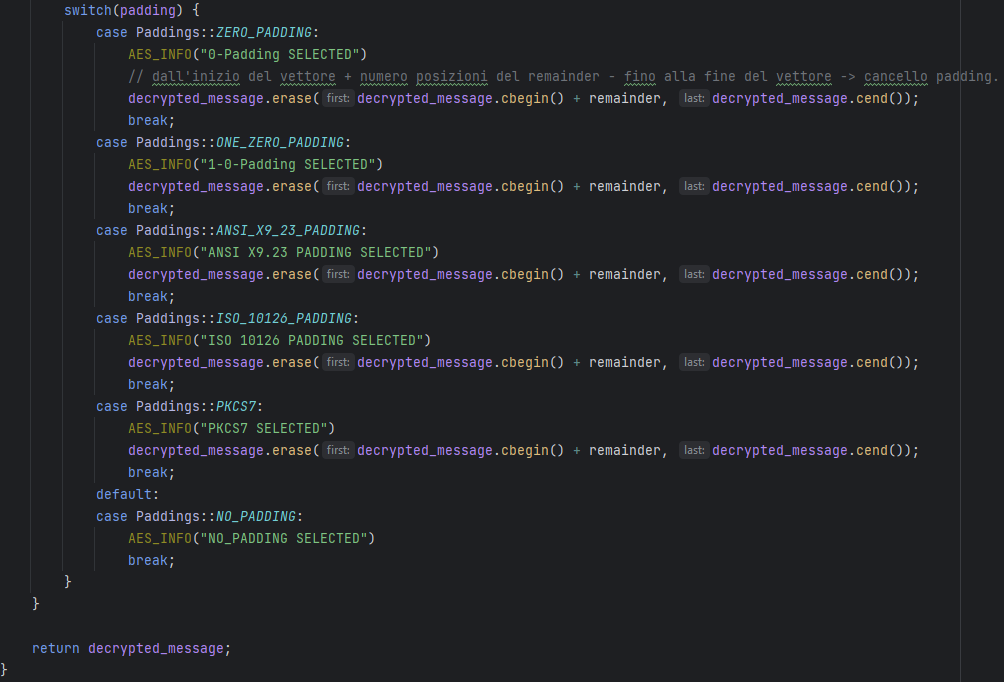
\includegraphics[width=1\textwidth, height=1\textheight, keepaspectratio]{./images/code/cpp/padding/remove_padding1.PNG}
	\caption{Rimozione del padding (2/2)}
	\label{fig:remove_padding1}
\end{figure}

\subsection{API}

\textsf{\small }

%TODO: solo encrypt e decrypt?

\subsubsection{Cifratura}

\textsf{\small }

\begin{figure}[H]
	\centering
	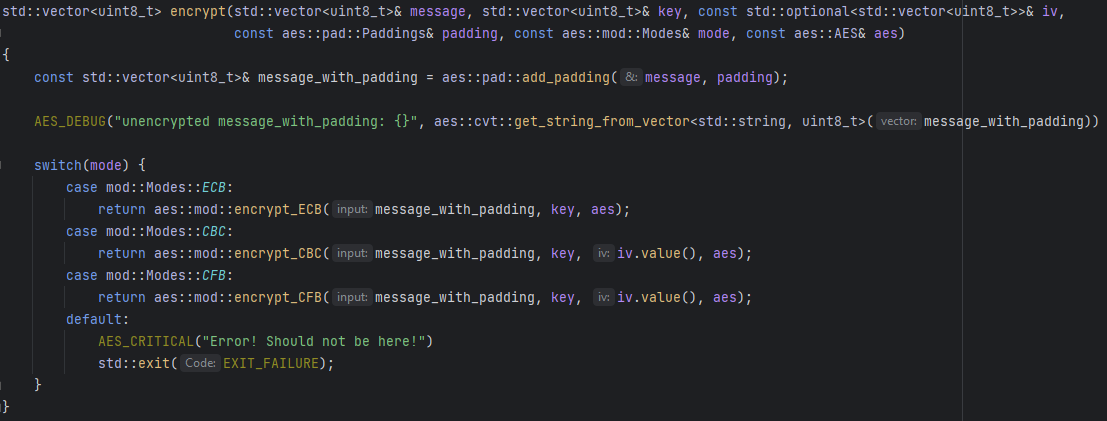
\includegraphics[width=1\textwidth, height=1\textheight, keepaspectratio]{./images/code/cpp/api/encrypt.PNG}
	\caption{Cifratura}
	\label{fig:encrypt}
\end{figure}

\subsubsection{Decifratura}

\textsf{\small }

\begin{figure}[H]
	\centering
	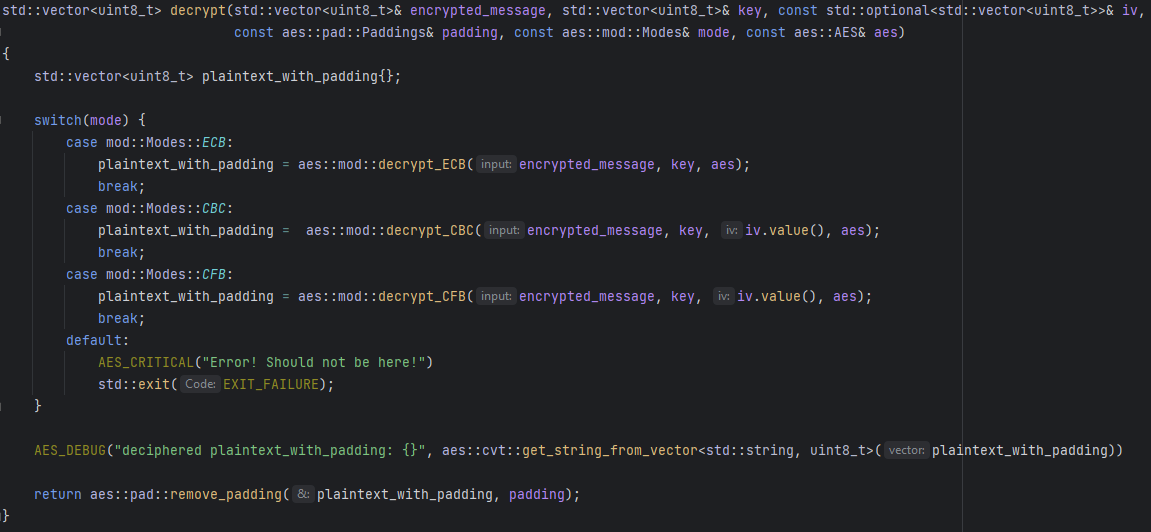
\includegraphics[width=1\textwidth, height=1\textheight, keepaspectratio]{./images/code/cpp/api/decrypt.PNG}
	\caption{Decifratura}
	\label{fig:decrypt}
\end{figure}

\textsf{\small } %TODO:

% ---------------------------- SECTION: IMPLEMENTAZIONE IN JAVA -------------------------

\section{Implementazione in Java}

\textsf{\small } %TODO: 

\begin{figure}[H]
	\centering
	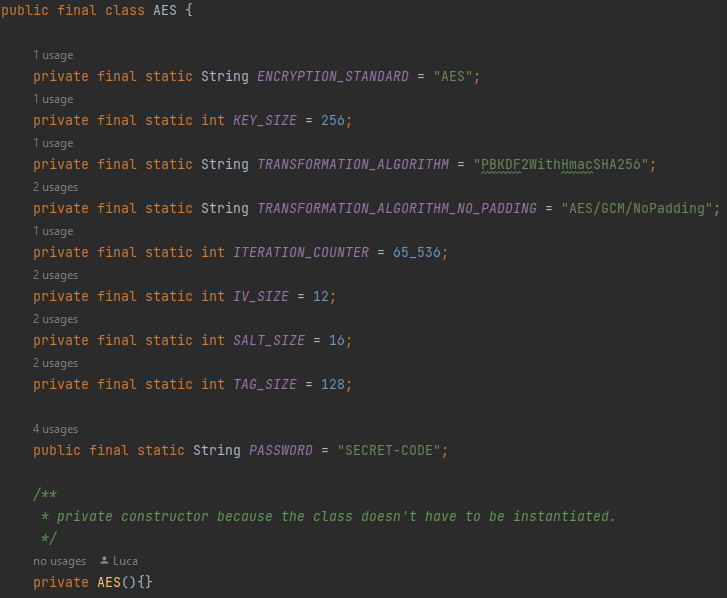
\includegraphics[width=1\textwidth, height=1\textheight, keepaspectratio]{./images/code/java/constructor_and_member_variables.PNG}
	\caption{Costruttore e variabili membre}
	\label{fig:constructor_and_member_variables}
\end{figure}

\textsf{\small } %TODO: 

\begin{figure}[H]
	\centering
	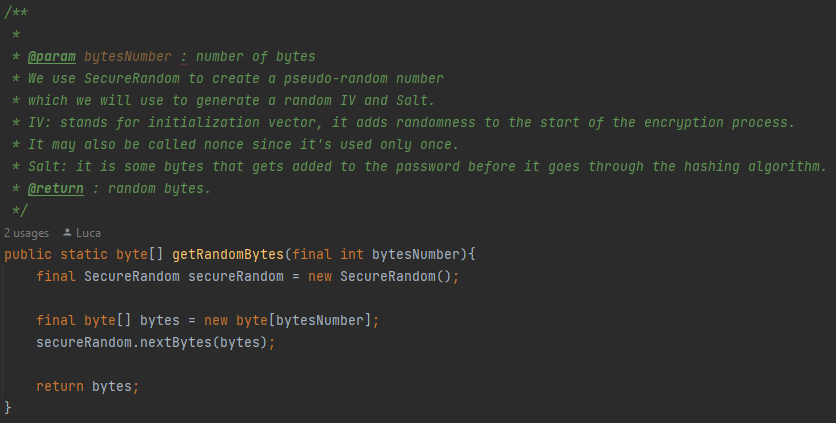
\includegraphics[width=1\textwidth, height=1\textheight, keepaspectratio]{./images/code/java/nonce_getRandomBytes.PNG}
	\caption{Nonce}
	\label{fig:nonce_getRandomBytes}
\end{figure}

\textsf{\small } %TODO: 

\begin{figure}[H]
	\centering
	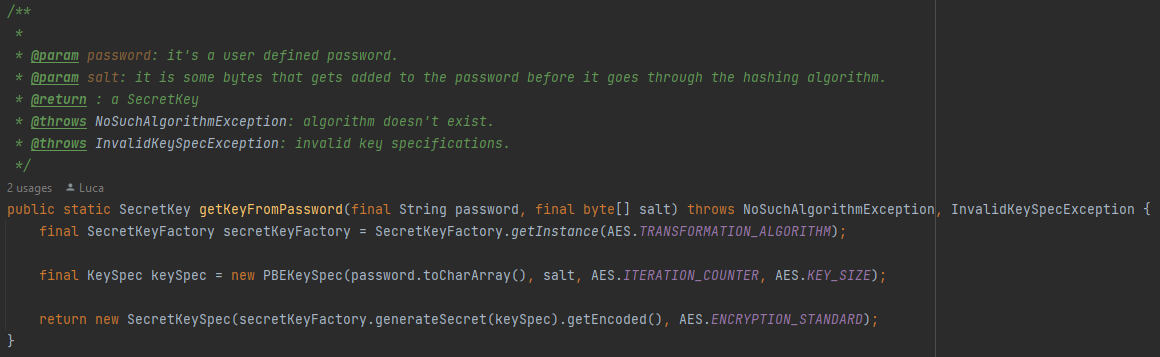
\includegraphics[width=1\textwidth, height=1\textheight, keepaspectratio]{./images/code/java/getKeyFromPassword.PNG}
	\caption{Password}
	\label{fig:getKeyFromPassword}
\end{figure}

\textsf{\small } %TODO: 

\begin{figure}[H]
	\centering
	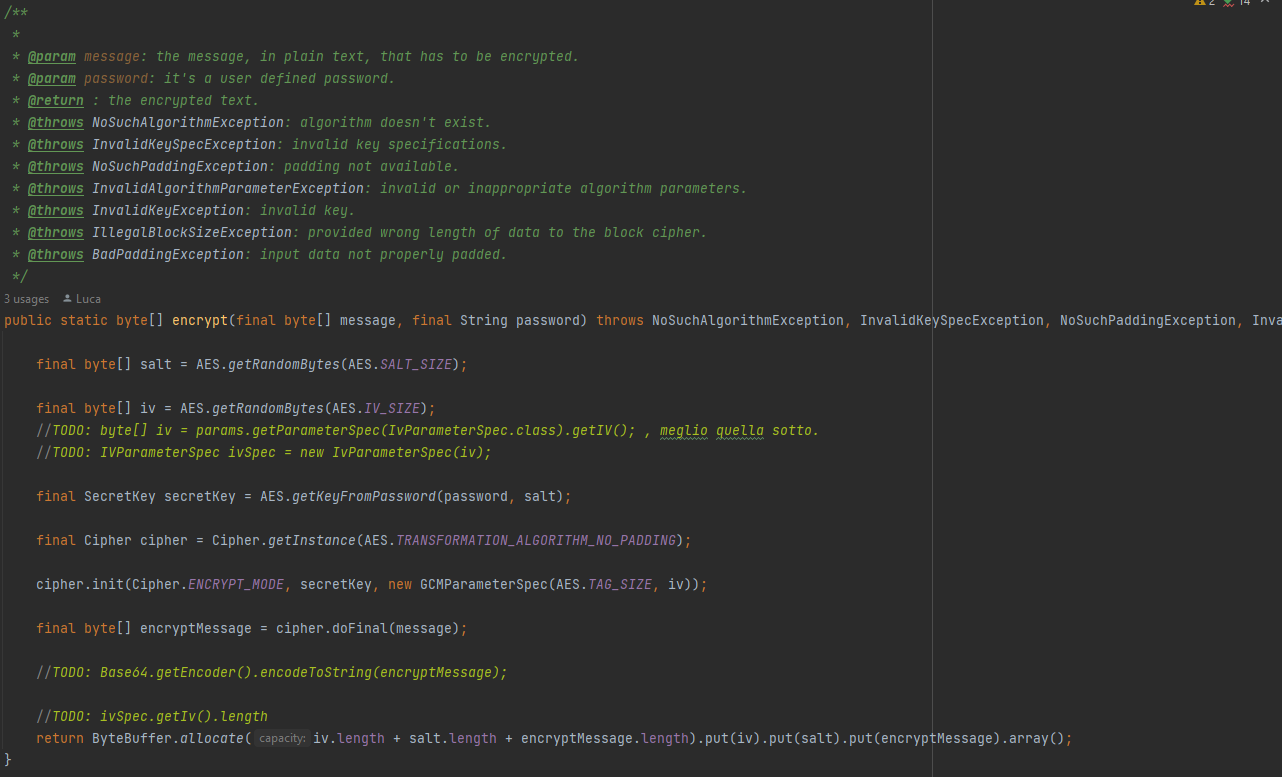
\includegraphics[width=1\textwidth, height=1\textheight, keepaspectratio]{./images/code/java/encrypt.PNG}
	\caption{Cifratura}
	\label{fig:encrypt_java}
\end{figure}

\textsf{\small } %TODO: 

\begin{figure}[H]
	\centering
	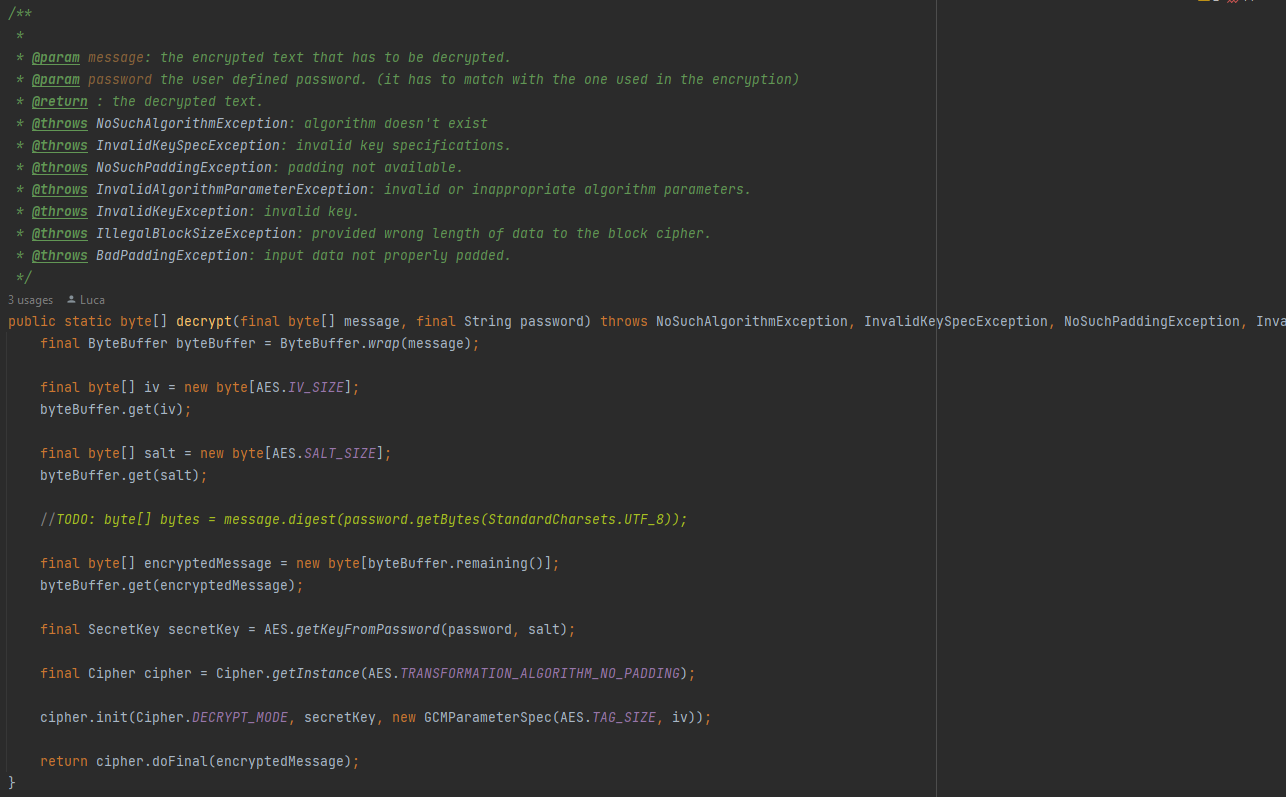
\includegraphics[width=1\textwidth, height=1\textheight, keepaspectratio]{./images/code/java/decrypt.PNG}
	\caption{Decifratura}
	\label{fig:decrypt_java}
\end{figure}

\textsf{\small } %TODO: 

\begin{figure}[H]
	\centering
	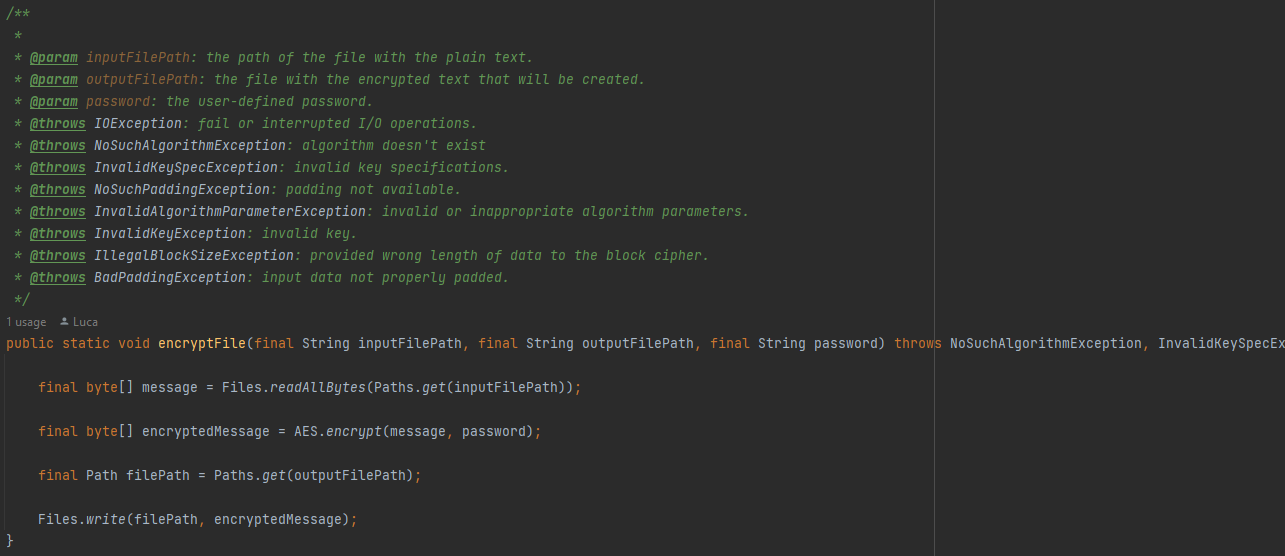
\includegraphics[width=1\textwidth, height=1\textheight, keepaspectratio]{./images/code/java/encryptFile.PNG}
	\caption{Funziona per la cifratura di un File}
	\label{fig:encryptFile}
\end{figure}

\textsf{\small } %TODO: 

\begin{figure}[H]
	\centering
	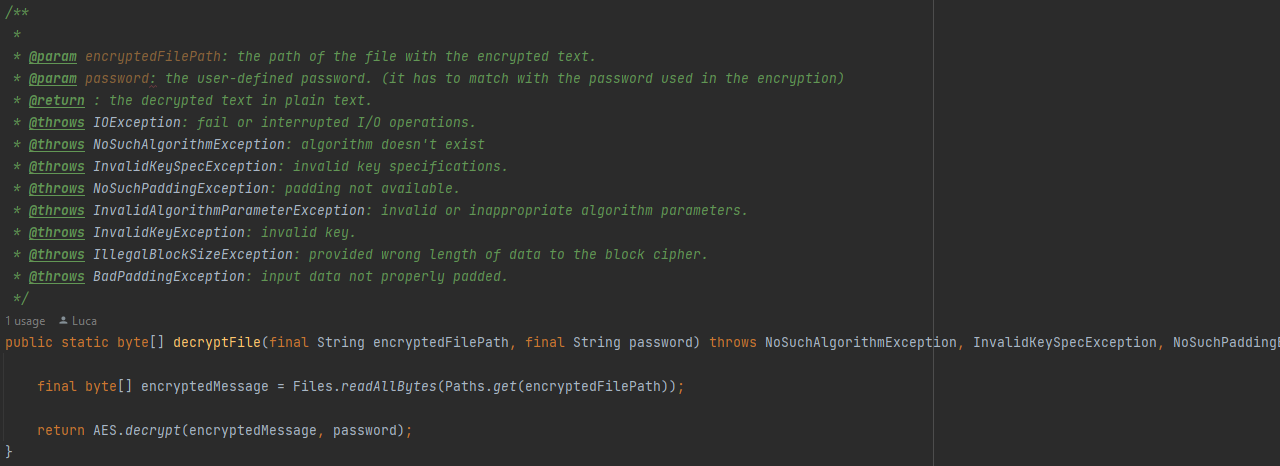
\includegraphics[width=1\textwidth, height=1\textheight, keepaspectratio]{./images/code/java/decryptFile.PNG}
	\caption{Funziona per la decifrazione di un File}
	\label{fig:decryptFile}
\end{figure}

\textsf{\small } %TODO: 

% -------------------------------- FINE CAPITOLO ----------------------------------------